\paginavaciacompleta
\chapter{iRprop+ en la aplicación Keel}\label{anexo}
A continuación exponemos el uso de la aplicación software Keel \footnote{http://www.keel.es}
(\textit{Knowledge Extraction based on Evolutionary Learning}) \cite{Keel2009} \noindent, en la
cual hemos introducido iRprop+, además de un nuevo módulo de enseñanza para el alumnado
interesado en el tipo de algoritmos y técnicas que ofrece la herramienta.

Keel permite ejecutar
múltiples AEs para problemas de minería de datos, incluyendo regresión,
clasificación, \textit{clustering}, etc. También contiene una gran colección de algoritmos clásicos
de extracción de conocimiento, técnicas de preprocesamiento (selección de características, selección
de instancias, discretización, métodos para el tratamiento de valores perdidos, etc), algoritmos de
aprendizaje basados en inteligencia computacional, incluyendo algoritmos evolutivos de
aprendizaje basados en reglas con diferentes aproximaciones (Pittsburgh, Michigan e IRL,...), así
como modelos híbridos como los sistemas difusos genéticos, ANNs evolutivas, etc. Keel
permite realizar un análisis completo de cualquier modelo de aprendizaje en comparación con otros
existentes, incluyendo un módulo estadístico para la comparación de
métodos.

Esta aplicación software ofrece varias ventajas. En primer lugar, se reduce el trabajo de
programación. Incluye una biblioteca con algoritmos evolutivos de aprendizaje basado en paradigmas
diferentes (Pittsburgh, Michigan e IRL) y simplifica la integración de múltiples algoritmos
evolutivos con diferentes técnicas de preprocesamiento. Esto puede aliviar a los investigadores del
mero "trabajo técnico" de la programación y que puedan centrarse más en el análisis de sus nuevos
modelos de aprendizaje en comparación con los ya existentes. En segundo lugar, se extiende el rango
de posibles usuarios de la aplicación con algoritmos evolutivos de aprendizaje. Una amplia
biblioteca de EAs, junto con un software fácil de usar, reduce considerablemente el nivel de
conocimiento y experiencia requeridos por los investigadores en computación evolutiva. Así,si
investigadores con menos conocimiento utilizan este aplicación software, serían capaces de
aplicar
con éxito los algoritmos de los que dispone Keel a sus problemas. En tercer lugar, debido al uso de
un enfoque orientado a objetos bajo el lenguaje Java, Keel se puede utilizar en cualquier máquina
con Java, independientemente del sistema operativo.

En lo que concierne a este anexo, hemos introducido en Keel el algoritmo iRprop+ que
 hemos usado como LS en nuestros algoritmos (ver sección
 \ref{rprop} del capítulo \ref{MOEANNs}). IRprop+ se ha introducido como método de clasificación de
 patrones utilizando ANNs, tanto con unidades SUs como PUs (ver sección
\ref{rprop} del  capítulo \ref{redesneuronales}). En Keel, se permite que iRprop+ se configure desde
la interfaz de
 usuario haciendo un doble clic sobre dicho método en la parte de diseño de experimentos (ver figura
 \ref{fig7aplica}). De esta manera hemos aportado un algoritmo de aprendizaje más al conjunto de
 algoritmos que ya poseía Keel, ampliando en este caso el numero de métodos existentes en Keel con
 ANNs. Todo ello se ha hecho haciendo una adaptación previa de iRprop+ sin cambiar su funcionalidad
 ni su rendimiento, para poder adaptarlo al tipo de entrada y salida que necesita Keel (algo que da
 mucha flexibilidad a la herramienta para que cualquiera pueda introducir su propio algoritmo).

Por otra parte, Keel se ha diseñado con un doble objetivo: científico y educacional. El
módulo científico está preparado para empaquetar un conjunto de algoritmos y conjuntos de datos
para que el usuario final pueda lanzarlos en una máquina externa, ya sea en un \textit{cluster} de
máquinas, o en un computador personal. El modulo educacional, del cual hemos sido unos de los
desarrolladores principales, permite prácticamente la misma funcionalidad que el módulo científico,
pero se ejecuta solo en la maquina local donde se esté usando, y permite seguir en tiempo de
ejecución el progreso de un algoritmo y los resultados que va obteniendo en cada instante. En la
figura \ref{fig5aplica} y \ref{fig6aplica} se pueden ver dos ejemplos de la parte de diseño de una
batería de pruebas en Keel, en la parte de investigación y en la parte educacional respectivamente.

En resumen, se ha ampliado el marco de trabajo de Keel con una parte educacional y con la
incorporación del algoritmo iRprop+ como método de aprendizaje con ANNS, ya se con
unidades de base
sigmoide o producto.

\begin{figure}[!h]
\centering
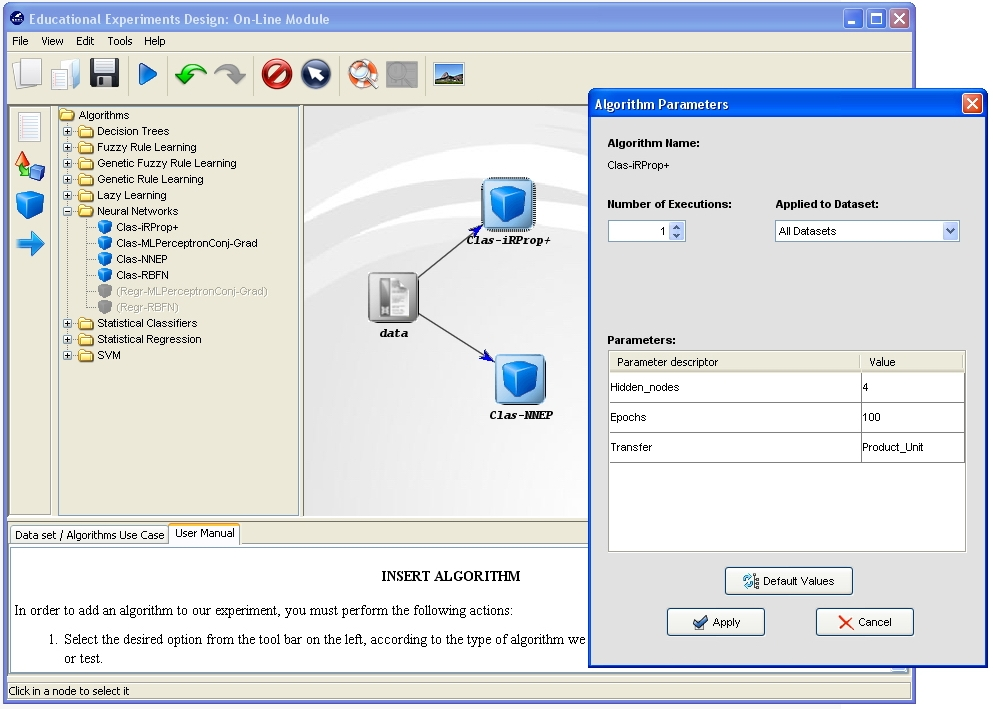
\includegraphics[keepaspectratio,width=12.7cm]{figuras/keel3.jpg}
\caption{Configuración del algoritmo iRprop+ en Keel usando 4 nodos en capa oculta con ANNs con
unidades de base producto y con 100 épocas.}
\label{fig7aplica}
\end{figure}

\begin{figure}[!h]
\centering
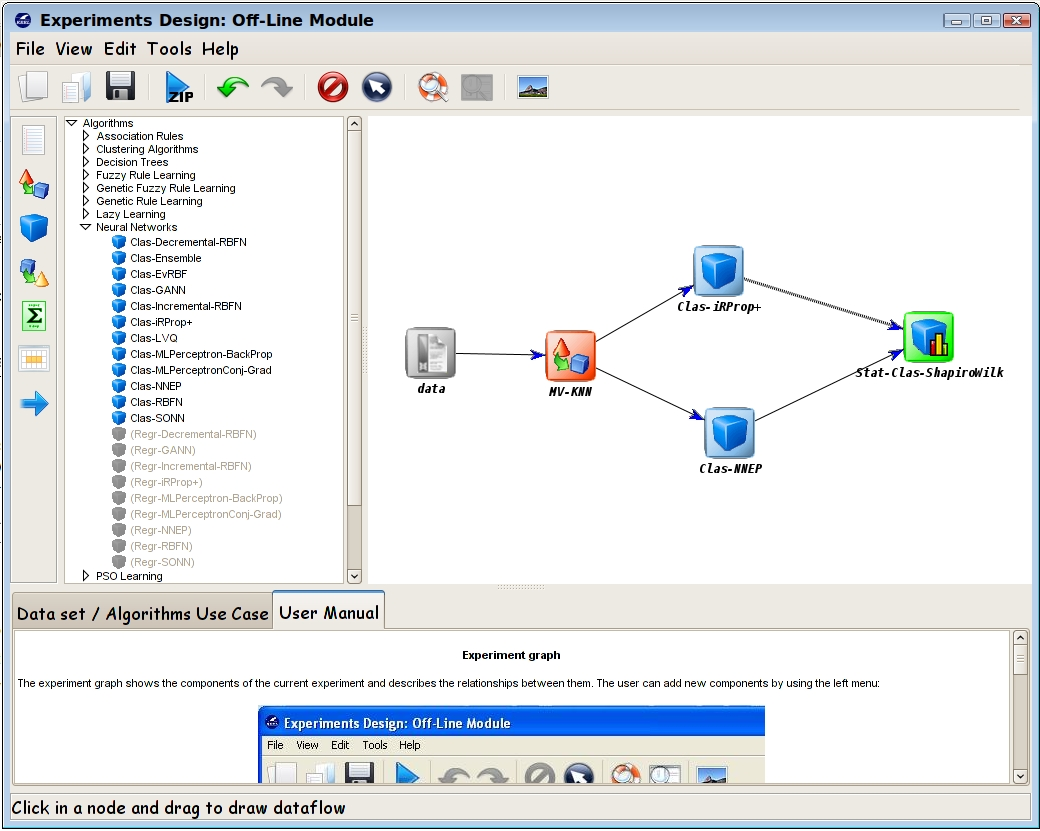
\includegraphics[keepaspectratio,width=12.7cm]{figuras/keel1.jpg}
\caption{Diseño experimental con dos algoritmos a evaluar en la parte científica de Keel.}
\label{fig5aplica}
\end{figure}
\paginavaciasincuerpo
\begin{figure}[!h]
\centering
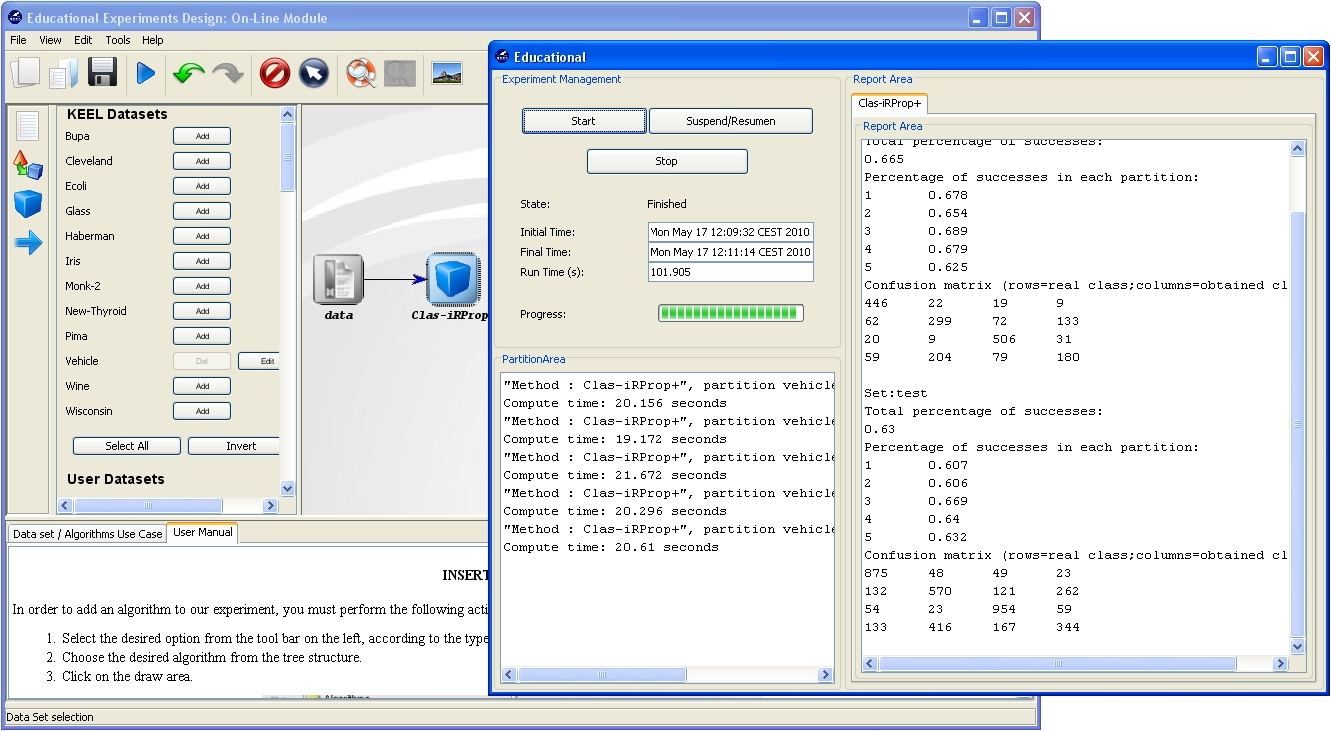
\includegraphics[keepaspectratio,width=12.7cm]{figuras/keel2.jpg}
\caption{Diseño experimental y ejecución de iRprop+ en la parte educacional de Keel.}
\label{fig6aplica}
\end{figure}
\paginavaciacompleta